\documentclass[polish,polish,a4paper]{article}
\usepackage[dvipsnames]{xcolor}
\usepackage[utf8]{inputenc}
\usepackage{polski}
\usepackage{tikz}
\usepackage{pgfplots}
\usepackage[margin = 1.in]{geometry}
\usepackage{subcaption}
\usepackage[export]{adjustbox}
\usepackage{hyperref}
\usepackage{tabularx}
\usepackage{mathtools}
\usepackage{multirow}
\usepackage{array}
\usepackage{hhline}
\usepackage{url}

\pgfplotsset{compat=1.16}
\newcommand{\name}[1]{\sffamily\bfseries\scriptsize #1}

\newcommand{\frontpage}[9]{
%% #1 - nazwa kursu
%% #2 - kierunek 
%% #3 - termin 
%% #4 - temat 
%% #5 - problem
%% #6 - skład grupy
%% #7 - brak
%% #8 - data
%% #9 - nr raportu
\noindent
\begin{tabularx}{\textwidth}{@{}X@{}l@{}}
    \begin{tabular}[t]{||m{0.5\textwidth}|m{0.25\textwidth}||}
        \hhline{|t:==:t|}
        \multicolumn{2}{||c||}{}\\
        \multicolumn{2}{||c||}{{\LARGE #1}}\\
        \multicolumn{2}{||c||}{}\\
        \hhline{||--||}
        \name{Kierunek} & \name{Termin}\\
        \textit{#2} & \textit{#3} \\
        \hhline{||--||}
        %\name{Imię, nazwisko, numer albumu} & \name{Nr laboratorium}\\
        %\textit{#6} & \textit{#5} \\
        \name{Imię, nazwisko, numer albumu} & \name{Data}\\
        \textit{#6} & \textit{#8} \\
        \hhline{||--||}
        %\name{Link do projektu} & \name{Data}\\
        %\url{#7} & \textit{#8} \\
        \multicolumn{2}{||l||}{\name{Link do projektu}} \\
        \multicolumn{2}{||l||}{\url{#7}} \\
        \hhline{|b:==:b|}
    \end{tabular}
    &
    
\includegraphics[width=2.25cm,valign=T]{images/PWr.png}
\end{tabularx}
\vspace{.5cm}

\begin{center}
    \LARGE \textsc{Raport #9}
\end{center}

\noindent\rule[0.5cm]{\textwidth}{1pt}
}
\begin{document}
\frontpage{%
    Programowanie Obiektowe% nazwa kursu
}{%
    Informatyka Techniczna% kierunek
}{%
    Środa TN 15:15% termin
}{-}{-}{%
    Bartosz Ostrowski 259222% dane osobowe
}{%
    https://www.overleaf.com/read/zvpwwmddrpkm% link do edytowalnej wersji projektu
}{24 czerwca 2021}{%
    % numer raportu
}
\pagestyle{empty}

\section{Jurassic Park}
\begin{center}
    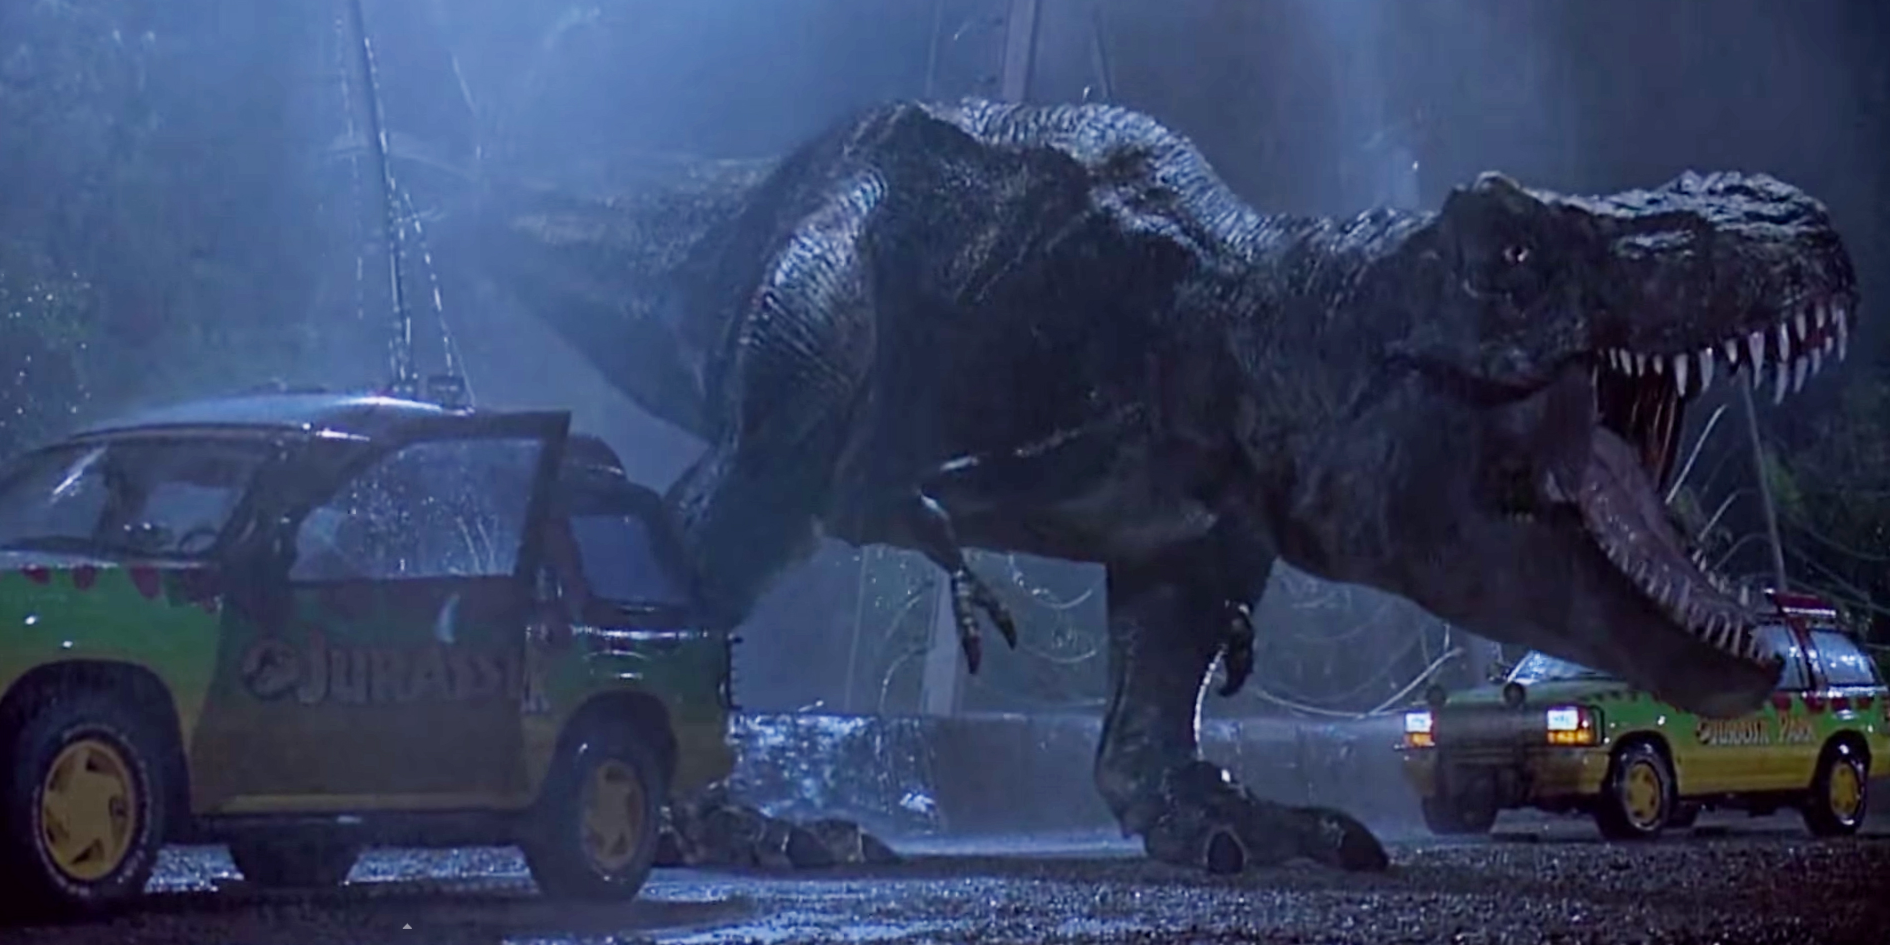
\includegraphics[width=0.7\columnwidth]{jurassic.png}
\end{center}
\subsection{Ogólne przedstawienie}
Symulacja będzie swoistą próbą przedstawienia filmowego Parku Jurajskiego, z głównym nastawieniem na cykl życia dinozaurów - podział na roślinożerność, wszystkożerność i mięsożerność. Ograniczoną listę dinozaurów opartą na encyklopedii (ów encyklopedia będzie zawarta w kodzie symulacja, będzie to lista określonych gatunków importowana z pliku dinosaurs.json). Plansza na której będzie się rozgrywać symulacja będzie losowo generować określone dinozaury. Na planszy dla roślinożerców powstanie obiekt będący reprezentacją ich jedzenia. Powstanie również obiekt wody - do napełniania pragnienia.
\subsection{Wartości startowe}
Będzie można określić prawdopodobieństwo wylosowania dinozaura i obiektu. Maksymalny rozmiar parku. Będzie też możliwa do ustawienia ilość iteracji, ile razy ma zostać wykonana cała plansza.
\subsection{Wstępne klasy}
\begin{enumerate}
    \item \textbf{Dinozaur} - będący główną klasą, mogący zawierać takie wartości jak: 
    \begin{itemize}
        \item gatunek z encyklopedii
        \item sposób odżywiania się (roślinożerność, wszystkożerność i mięsożerność)
        \item zdrowie - gatunki mięsożerne będą musiały polować, przykładowo zdrowie 0 oznacza zwłoki/padlinę występującą na planszy
        \item głód - w przypadku spadnięcia do 0, dostaje obrażenia w każdej następnej iteracji
        \item pragnienie - uzupełniane przy złożach wody na planszy, w przypadku spadnięcia do 0 dostaje obrazenia w każdej następnej iteracji
        \item szybkość - każdy dinozaur charakteryzuje się inną szybkością
    \end{itemize}
    \item \textbf{Rośliny} - obiekt głównie do jedzenia dla roślinożerców:
    \begin{itemize}
        \item ilość w jednym obiekcie
    \end{itemize}
    \item \textbf{Woda} - obiekt głównie do napełniania pragnienia dla wszystkich typów dinozaurów
    \begin{itemize}
        \item ilość w jednym obiekcie
    \end{itemize}
\end{enumerate}
\subsection{Koniec symulacji}
Symulacja kończy się po określonej liczbie iteracji.

\section{Analiza czasownikowo-rzeczownikowa}
Projektujemy symulację agentowa, która będzie badać zachowanie \textcolor{blue}{dinozaurów} \textcolor{blue}{różnych gatunków}. Symulacja będzie zawierać \textcolor{blue}{planszę dwuwymiarową (X,Y) o zadanej wielkości}, gdzie na \textcolor{orange}{każdym jednym polu powstanie} obiekt \textcolor{blue}{rośliny}, \textcolor{blue}{wody}, \textcolor{blue}{dinozaura}, bądź \textcolor{blue}{pustego pola (tzw. Tile)}.
\begin{itemize}
    \item Zachowanie się dinozaurów:
    \begin{itemize}
        \item W zależności od \textcolor{blue}{gatunku dinozaur} może \textcolor{orange}{jeść} określone \textcolor{blue}{pożywienie} - \textcolor{blue}{rośliny}, albo \textcolor{blue}{innego dinozaura} (gdzie dinozaur "je" innego, tylko podczas ataku, zwracana jest adekwatna ilość głodu do ataku, dinozaur może atakować martwego, co też daje mu pożywienie), bądź to i to, \textcolor{orange}{zapełniając w ten sposób} \textcolor{blue}{głód}.
        \item \textcolor{blue}{Mięsożercy}, oraz \textcolor{blue}{wszystkożercy} mogą \textcolor{orange}{atakować dinozaury innego gatunku, co skutkuje obniżeniem zdrowia atakowanego dinozaura o określoną wartość i uzupełnia lekko głód atakującego}.
        \item Podobnie z \textcolor{blue}{pragnieniem}, tylko \textcolor{orange}{uzupełnianie go} będzie przy polach \textcolor{blue}{wód}.
        \item Na starcie symulacji \textcolor{blue}{dinozaury} \textcolor{orange}{pojawiają się w losowych polach}.
        \item \textcolor{orange}{Dinozaury poruszają się w losowym kierunku, o określoną w gatunku liczbę pól}. Mogą dostać się tylko na nieoblegane \textcolor{blue}{pole} i \textcolor{orange}{wykonać możliwą akcję} z \textcolor{blue}{polem sąsiadującym PO RUCHU}.
    \end{itemize}
    \item Pola \textcolor{blue}{rośliny}, \textcolor{blue}{wód} i \textcolor{blue}{pól (tzw. Tile)} są statyczne, \textcolor{orange}{nie poruszają się}, mogą być tylko \textcolor{orange}{użyte przez dinozaury}.
    \item Parametry symulacji:
        \begin{itemize}
            \item Wielkość przestrzeni S*S.
            \item Importowana z pliku dinosaurs.json - n liczba gatunków
            \item Prawdopodobieństwo pojawienia się elementu (element, to statyczne obiekty czyli roślina, woda bądź puste pole) $E_r$.
            \item Prawdopodobieństwo pojawienia się dinozaura (losowany jest z importowanej listy (encyklopedii), więc nie ma zasady pojawienia się więcej danego typu) $D_r$.
            \item Gdzie $\sum E_r + D_r + x = S*S$, gdzie x to pozostałe puste niezamieszkane pola.
            \item Maksymalna liczba iteracji I.
        \end{itemize}
\end{itemize}
\newpage
\section{Diagramy UC}
    \begin{figure}[h!]
        \centering
        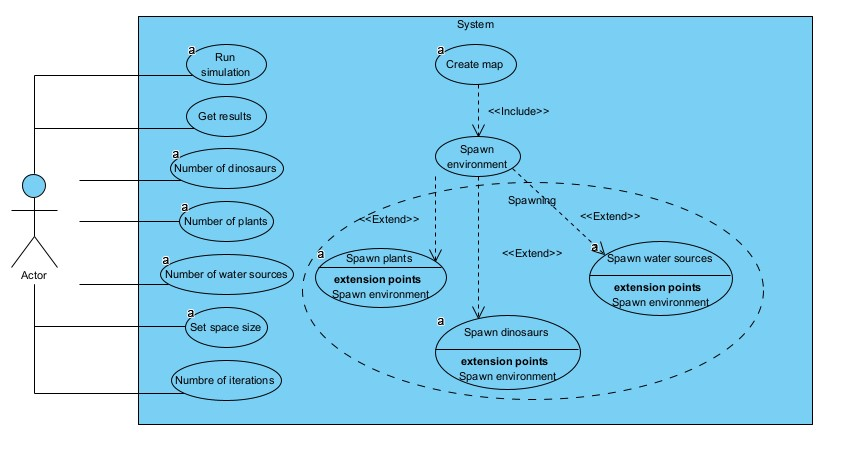
\includegraphics[scale=0.65]{images/usecase/use_case1.jpg}
        \caption{Diagram UC - ustawienia i opcje użytkownika oraz tworzenie mapy.}
        \label{fig:uc}
    \end{figure}
    
    \begin{figure}[h]
        \centering
        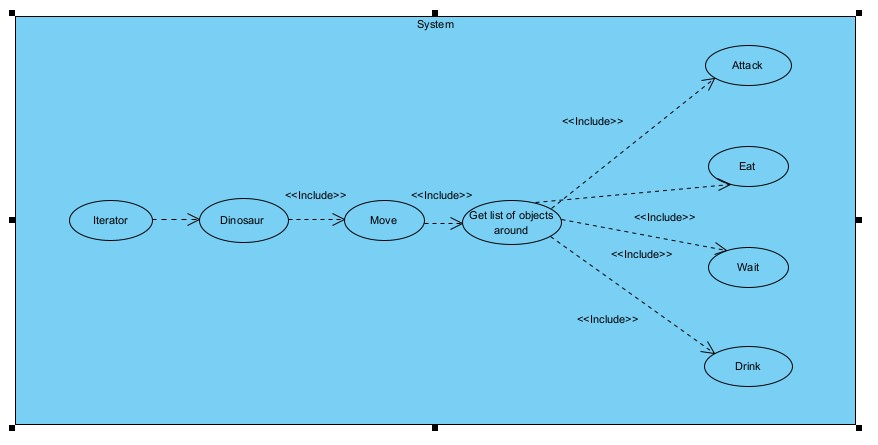
\includegraphics[scale=0.65]{images/usecase/use_case2.jpg}
        \caption{Diagram UC - poglądowe działanie systemu.}
        \label{fig:my_label}
    \end{figure}
\newpage 
\section{Karty CRC}
\subsection{Interfejsy}
\begin{figure}[h]
    \centering
    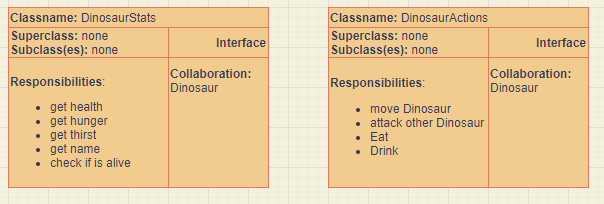
\includegraphics{images/crc/interfaces.png}
    \caption{Interfejsy do obsługi metod klasy Dinosaur.}
    \label{fig:interface}
\end{figure}

\subsection{Klasy abstrakcyjne}
W tym wypadku klasa abstrakcyjna Dinosaur może dziedziczyć po dwóch interfejsach (zgodnie z dokumentacją Javy - Klasa może dziedziczyć tylko po jednej Klasie, ale interfejsy są wyjątkiem).

\begin{figure}[h!]
    \centering
    \begin{minipage}{0.45\textwidth}
        \centering
        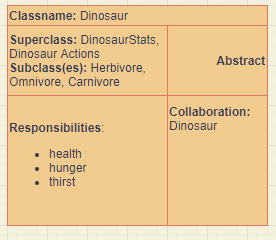
\includegraphics[width=0.9\textwidth]{images/crc/abs.png} % first figure itself
        \caption{Klasa abstrakcyjna Dinosaur.}
    \end{minipage}\hfill
    \begin{minipage}{0.45\textwidth}
        \centering
        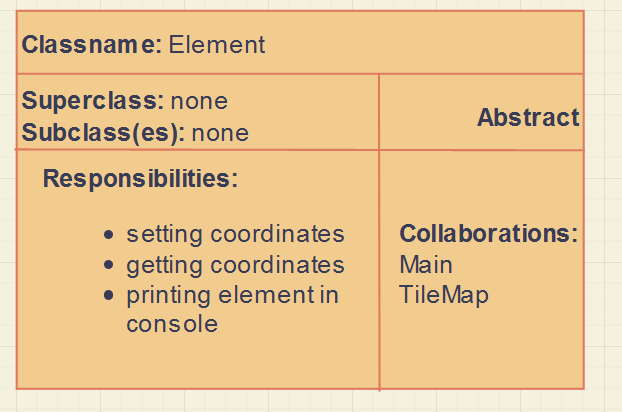
\includegraphics[width=0.9\textwidth]{images/crc/crc_element.png} % second figure itself
        \caption{Klasa abstracyjna Element.}
    \end{minipage}
\end{figure}

\newpage
\subsection{Klasy}
\begin{figure}[h!]
    \centering
    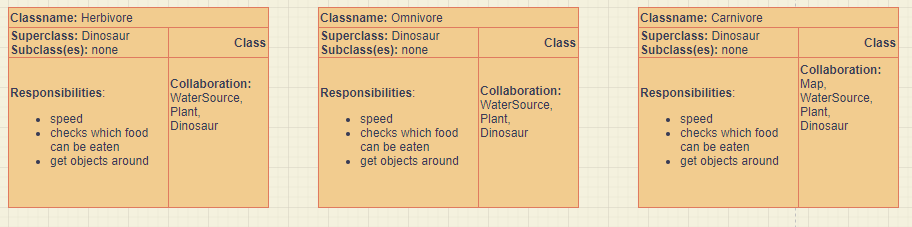
\includegraphics[scale=0.75]{images/crc/dinosaur_types.png}
    \caption{Klasy dziedziczące po klasie abstrakcyjnej Dinosaur.}
    \label{fig:klasa1}
\end{figure}

\begin{figure}[h!]
    \centering
    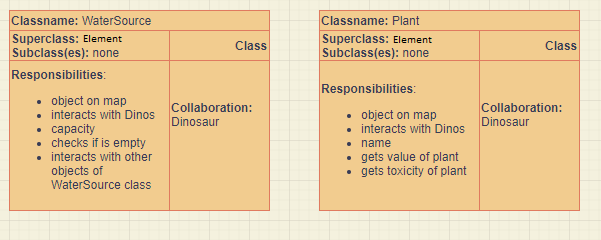
\includegraphics[scale=0.75]{images/crc/map_elements.png}
    \caption{Klasy będące elementami mapy.}
    \label{fig:my_label}
\end{figure}

\begin{figure}[h!]
    \centering
    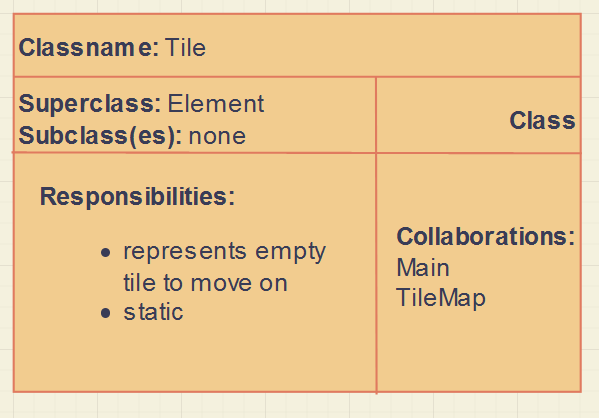
\includegraphics[scale=0.75]{images/crc/tiles_crc.png}
    \caption{Klasa będąca elementem mapy.}
    \label{fig:}
\end{figure}

\begin{figure}[h]
    \centering
    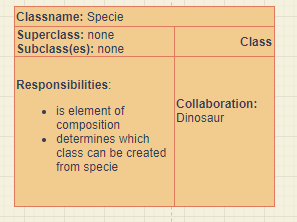
\includegraphics[scale=0.75]{images/crc/specie.png}
    \caption{Klasa która zawiera się w klasie abstrakcjnej Dinosaur (kompozycja).}
    \label{fig:specie}
\end{figure}

\newpage

\begin{figure}[h!]
    \centering
    \begin{minipage}{0.45\textwidth}
        \centering
        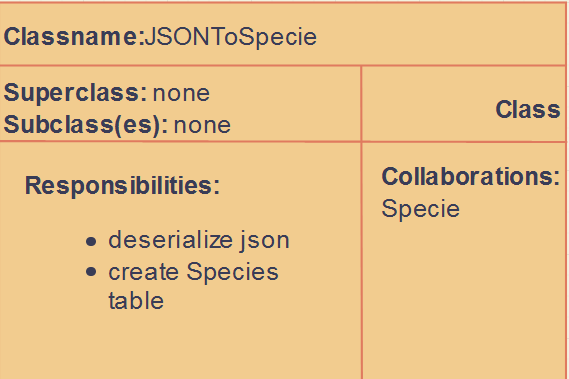
\includegraphics[width=0.9\textwidth]{images/crc/crc_json} % first figure itself
        \caption{Klasa do obsługi deserializacji plików JSON.}
    \end{minipage}\hfill
    \begin{minipage}{0.45\textwidth}
        \centering
        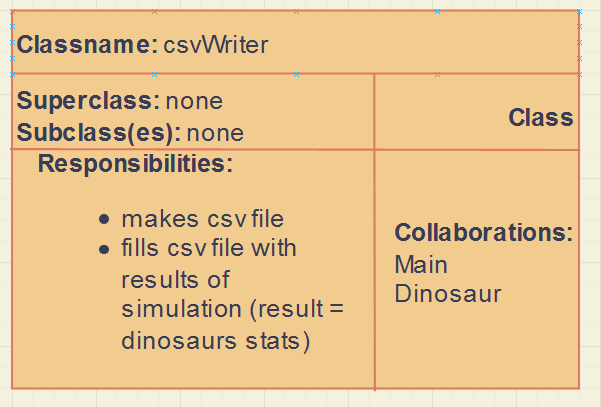
\includegraphics[width=0.9\textwidth]{images/crc/csv_crc.png} % second figure itself
        \caption{Klasa do eksportu do CSV.}
    \end{minipage}
\end{figure}

\begin{figure}[h!]
    \centering
    \begin{minipage}{0.45\textwidth}
        \centering
        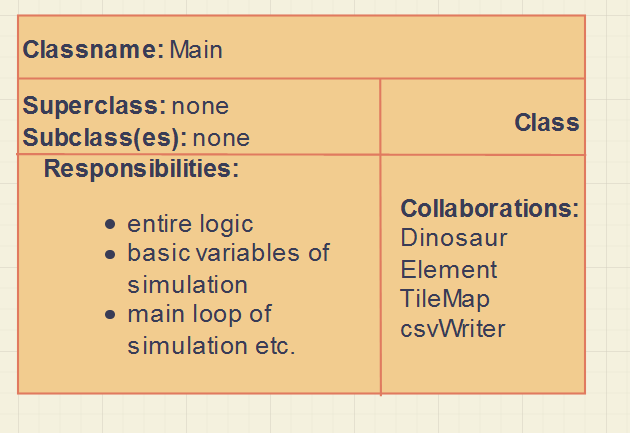
\includegraphics[width=0.9\textwidth]{images/crc/main_crc.png} % first figure itself
        \caption{Główna klasa.}
    \end{minipage}\hfill
    \begin{minipage}{0.45\textwidth}
        \centering
        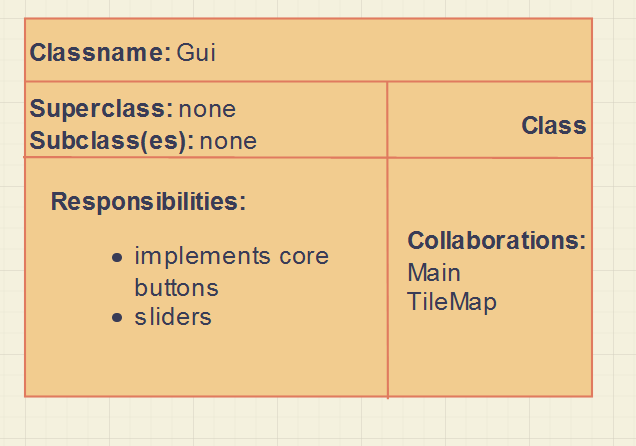
\includegraphics[width=0.9\textwidth]{images/crc/gui_crc.png} % second figure itself
        \caption{Klasa do utworzenia GUI.}
    \end{minipage}
\end{figure}

\begin{figure}[h!]
    \centering
    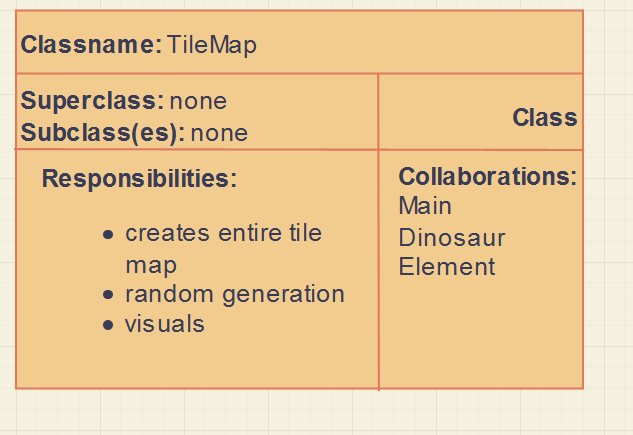
\includegraphics[scale=0.75]{images/crc/tilemap_crc.png}
    \caption{Klasa reprezentująca główną mapę kafelkową.}
    \label{fig:my_label}
\end{figure}

\newpage

\section{Diagramy Klas}
Zaznaczając jeszcze polimorfizm jest zastosowany nie tylko jako metoda w Canivore, Omnivore i Hebivore - mowa o getSpecieName(), stosuje także polimorfim, już w głównym kodzie w klasie Main, tam mam ustawione przykładowe działania:
\begin{itemize}
    \item dino instanceof Carnivore - wtedy porusza się o 3 pola
    \item dino instanceof Omnivore - wtedy porusza się o 2 pola
    \item etc...
\end{itemize}

Poniżej diagramy klas, okazały się być bardzo rozbudowane, więc możliwe, że są słabo widoczne na niektórych wyświetlaczach, dlatego w archiwum głównym \textit{ostrowski.zip} można je znaleźć \\ pod \textit{wszystkie\_klasy.png}
\newpage
\begin{figure}[h!]
    \centering
    \begin{minipage}{0.45\textwidth}
        \centering
        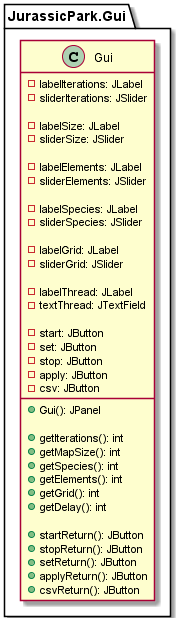
\includegraphics[width=0.9\textwidth]{images/class/gui.png} % first figure itself
        \caption{Układ pakietu Main.}
    \end{minipage}\hfill
    \begin{minipage}{0.45\textwidth}
        \centering
        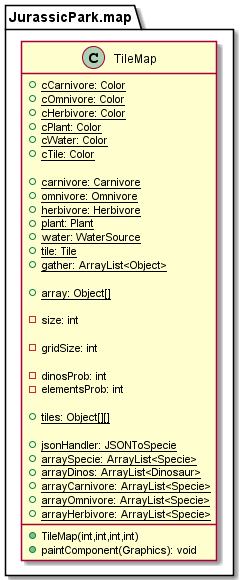
\includegraphics[width=0.9\textwidth]{images/class/map.png} % second figure itself
        \caption{Układ pakietu Map.}
    \end{minipage}
\end{figure}

\begin{figure}[h!]
    \centering
    \begin{minipage}{0.45\textwidth}
        \centering
        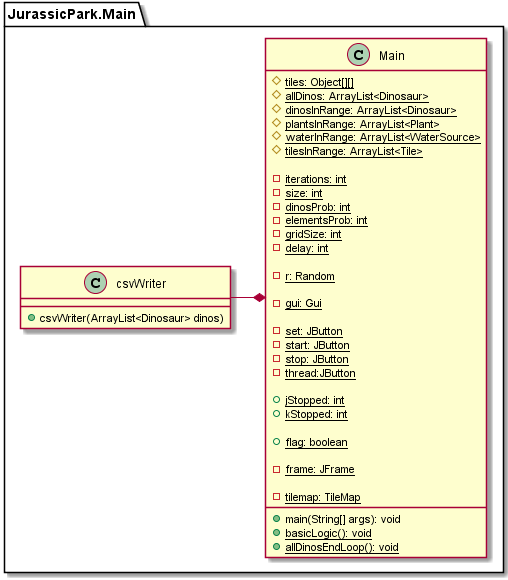
\includegraphics[width=0.9\textwidth]{images/class/main.png} % first figure itself
        \caption{Układ pakietu Gui.}
    \end{minipage}\hfill
    \begin{minipage}{0.45\textwidth}
        \centering
        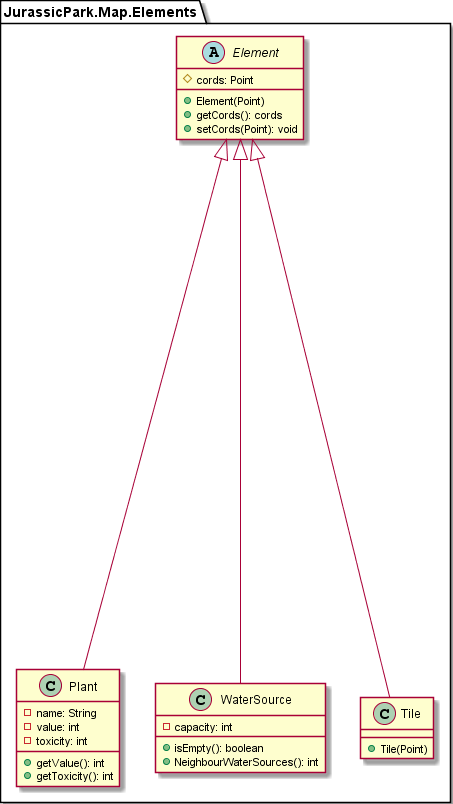
\includegraphics[width=0.9\textwidth]{images/class/elements.png} % second figure itself
        \caption{Układ pakietu Map.Elements.}
    \end{minipage}
\end{figure}

\newpage
\section{Diagramy obiektów}

\begin{figure}[h!]
    \centering
    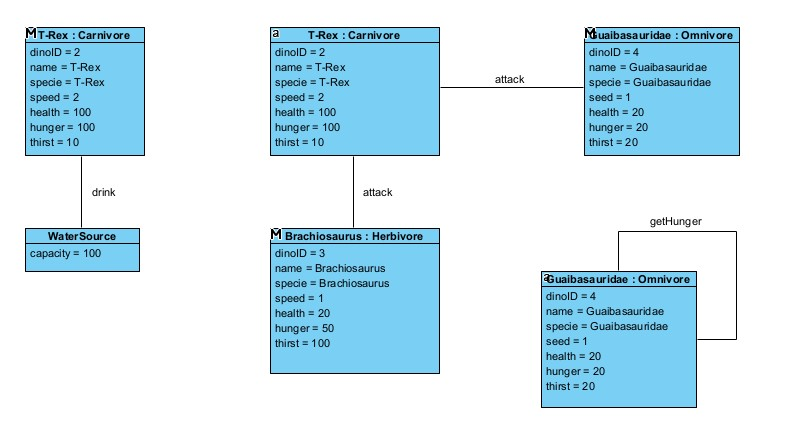
\includegraphics[scale=0.70]{images/object/object_diagram_1.jpg}
    \caption{Diagram obiektów - przykład losowych akcji podczas jednej iteracji (mało szczegółowe)}
    \label{fig:obj1}
\end{figure}


\begin{figure}[h!]
    \centering
    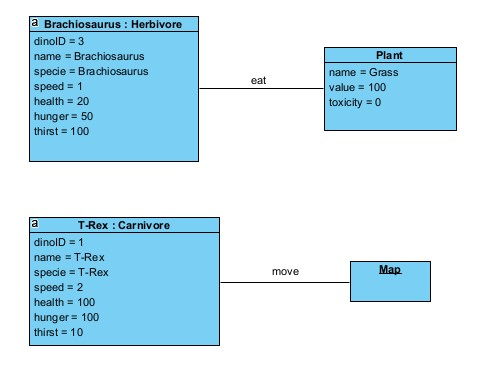
\includegraphics[scale=0.70]{images/object/object_diagram_2.jpg}
    \caption{Diagramy obiektów - dalsze przykłady losowych akcji.}
    \label{fig:obj2}
\end{figure}
\newpage
\begin{figure}[h]
    \centering
    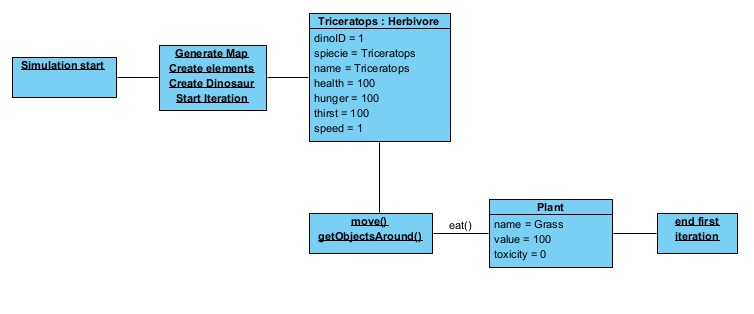
\includegraphics[scale=0.70]{images/object/object_diagram_3.jpg}
    \caption{Diagram obiektów - prezentujący poglądowo pierwszą startową iterację.}
    \label{fig:my_label}
\end{figure}

\newpage
\section{Diagram/diagramy sekwencji}

\begin{figure}[h!]
    \centering
    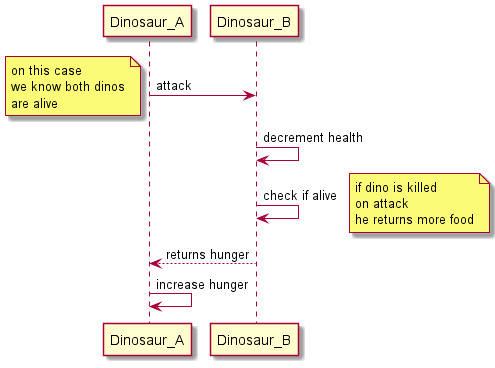
\includegraphics[scale=0.55]{images/sequence/sequence_attack.png}
    \caption{Diagram prezentujący sekwencje ataku.}
    \label{fig:sattack}
\end{figure}

\begin{figure}[h!]
    \centering
    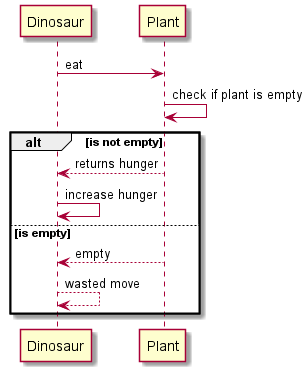
\includegraphics[scale=0.64]{images/sequence/sequence_eat.png}
    \caption{Diagram prezentujący sekwencje pożywiania się roślinami.}
    \label{fig:seat}
\end{figure}
\newpage
\begin{figure}[h!]
    \centering
    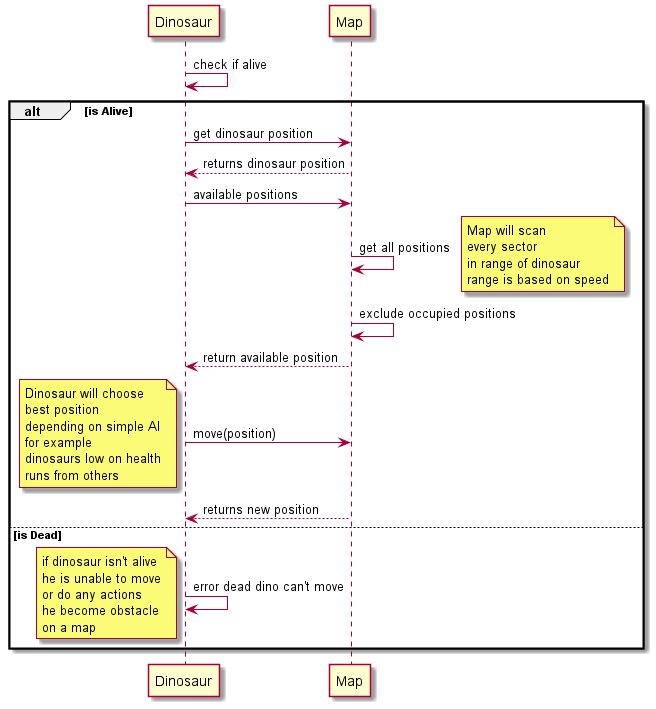
\includegraphics[scale=0.67]{images/sequence/sequence_move.png}
    \caption{Diagram prezentujący sekwencje poruszania się dinozaura.}
    \label{fig:smove}
\end{figure}
\newpage
\section{Diagram/diagramy aktywności}
Uznałem tutaj, że aktywnością może też być generowanie obiektów na mapie w całej symulacji. Wszelkie aktywności odwołują się bardzo ogólnie do stworzonych (do poprzedniego zadania) klas.
\begin{figure}[h]
    \centering
    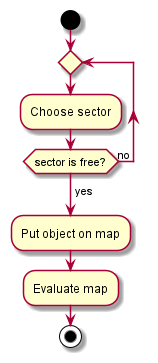
\includegraphics[scale=0.58]{images/activity/activity_generating.png}
    \caption{Diagram prezentujący generowanie obiektów na mapie.}
    \label{fig:agenerating}
\end{figure}

\begin{figure}[h]
    \centering
    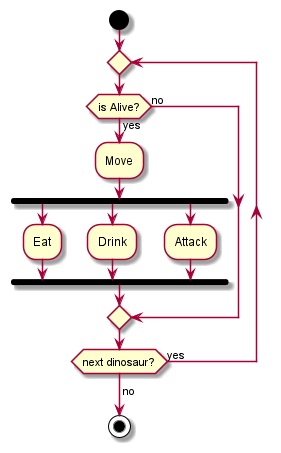
\includegraphics[scale=0.58]{images/activity/activity_interation.png}
    \caption{Diagram prezentujący możliwe aktywności dinozaura w iteracjach.}
    \label{fig:aiteration}
\end{figure}

\newpage
\newpage
\section{Diagram/diagramy maszyny stanów}

\begin{figure}[h!]
    \centering
    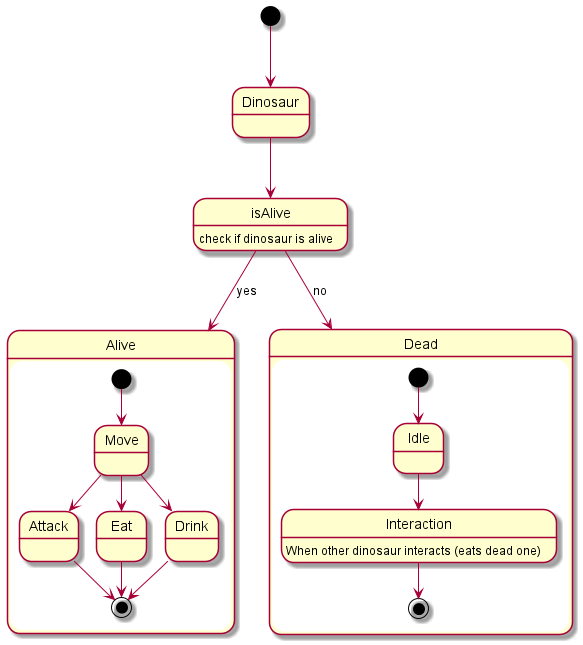
\includegraphics[scale=0.65]{images/state/state_alive.png}
    \caption{Diagram prezentujący stany życia dinozaura i określone dla nich akcje.}
    \label{fig:stalive}
\end{figure}
\newpage
\begin{figure}[h!]
    \centering
    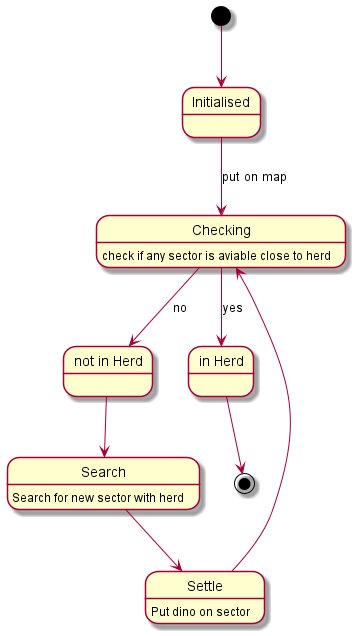
\includegraphics[scale=0.65]{images/state/state_herds.png}
    \caption{Diagram prezentujący stany czy dany dinozaur jest w stadzie czy nie.}
    \label{fig:stherds}
\end{figure}
\newpage

\section{Dokumentacja}

Pełną dokumentację można znaleźć w folderze \textit{JurassicPark/doc} - wygenerowana w pełni javadoc'em, na podstawie komentarzy z kodu programu.

\section{Dodatkowe elementy}

\subsection{GUI}
Dla wszelkich nieścisłości przygotowałem krótki opis działania GUI:
\begin{figure}[h]
    \centering
    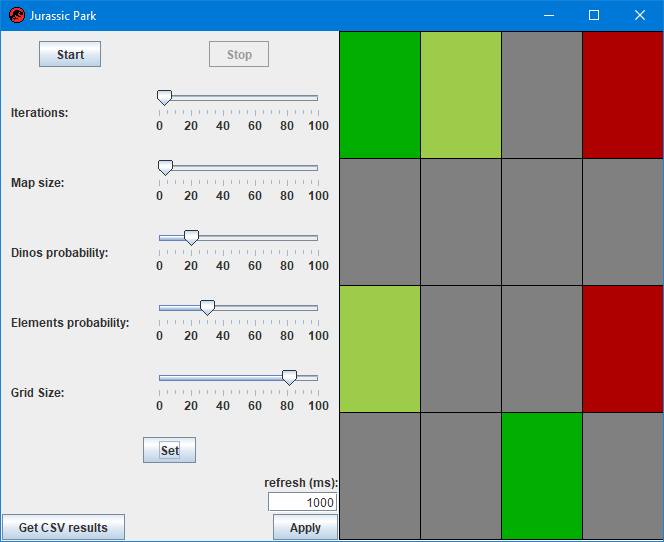
\includegraphics[scale=0.80]{images/gui.png}
    \caption{Zdjęcie podglądowe GUI}
    \label{fig:GUI}
\end{figure}

\begin{itemize}
    \item start - jak sama nazwa wskazuje, startuje symulacje (thanks captain obvious) - przycisk startu można kliknąć tylko wtedy kiedy symulacja nie jest w trakcie, oraz przycisk start blokuje "set", lecz nie blokuje sliderów.
    \item stop - przycisk stopu działa tylko gdy symulacja jest uruchomiona
    \item set - możemy w każdej chwili tym przyciskiem wygenerować nową planszę, zgarnia on wszystkie dane z suwaków wyżej (powinienem był przygotować jeszcze przycisk restartu, żeby nie losowało nowej symulacji, ale zabrakło czasu)
    \item get csv results - tworzy i zapisuje wszystkie dinozaury do pliku \textit{Simulation\_Results.csv}
    \item apply - służy do zmieniania opóźnienia w wykonywaniu się głównej pętli, domyślna wartość 1000ms, czyli po 1 sekundzie, przeskakujemy na kolejne pole.
    \item suwak iterations - dobieramy ile razy ma wykonać się pętla sprawdzająca wszystkie pola na mapie (lepszym rozwiązaniem byłoby pole do wprowadzania liczby, jak na "refresh - apply", ale wtedy okienko gorzej wygląda)
    \item suwak map size - wielkość planszy $S^2$
    \item suwak dinos probability i elements probability - brak blokady na ustawienie 100\% wystepowania obu zestawów elementów, co może skutkować dziwnymi generowaniami, polecam trzymać się w okolicach danych jak na obrazku
    \item grid size - rozmiar każdego pola
\end{itemize}
\subsection{Odczytywanie z pliku JSON dinozaurów}

Odczytywanie plików JSON, wykorzystałem do tego bibliotekę Google GSON, plik odczytywany to: \textit{JurassicPark/src/main/resources/dinosaurs.json}

\begin{figure}[h!]
    \centering
    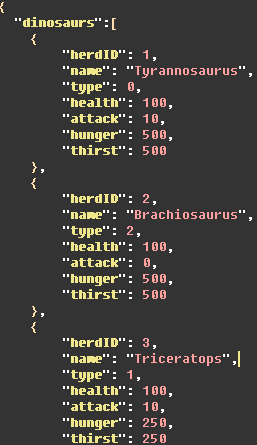
\includegraphics{images/json.png}
    \caption{podgląd pliku dinosaurs.json}
    \label{fig:json}
\end{figure}

Zgodnie ze schematem ustawiamy po kolei:
\begin{itemize}
    \item herdID - służy do identyfikowania konkretnych gatunków, liczba całkowta
    \item name - nazwa, może się powtarzać
    \item type - od 0 do 2, gdzie 0 to Carnivore, 1 to Omnivore i 2 to Herbivore
    \item health - liczba całkowita
    \item attack - liczba całkowita
    \item hunger - liczba całkowita
    \item thirst - liczba całkowita
\end{itemize}

Ostrzegam, trzeba się trzymać zasad wprowadzania, nie stworzyłem kontroli błędów, więc jeśli \textit{type} podamy inny niż 0, 1 lub 2, to możliwe, że program przestanie działać.

\newpage
\subsection{Eksport do CSV}

Zapisywanie wyników symulacji do pliku CSV o nazwie \textit{Simulation\_Results.csv}, zaimplementowałem tylko zapisywanie wszystkich dinozaurów i ich statystyk.

\begin{figure}[h!]
    \centering
    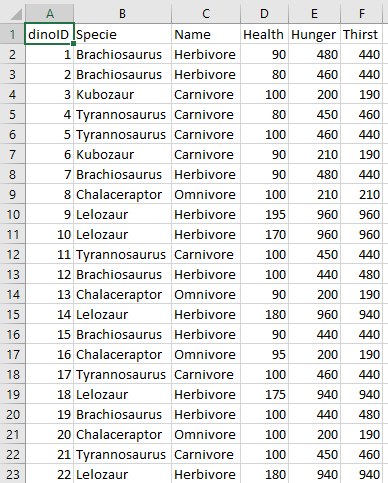
\includegraphics{images/csv.png}
    \caption{Podglądowy wygląd wyeksportowanego pliku.}
    \label{fig:my_label}
\end{figure}
\end{document}

